The aim of the proposed system is to investigate the implementation of \gls{coap} 
on a \gls{rpi} and how \gls{coap} can be used to transmit data to the cloud. 

To achieve this, a \gls{coap} endpoint will need to be created on the \gls{rpi}. 
The \gls{rpi} will collect sensor data at intervals and store them 
locally on the device. The \gls{rpi} will act as a \gls{coap} endpoint that will 
send to \gls{rest} POST requests with the sensor data and the time
the reading was taken in a \gls{json} format.

The clouds responsibility will be to receive the POST requests from the \gls{coap} 
endpoint hosted on the \gls{rpi} and to store and format the data. 
The cloud should send an Acknowledgement message to the \gls{coap} endpoint, 
containing a 2.01 (Created) Response Code or a 2.04 (Changed) Response Code 
and the URI of the created / updated resource \citep{shelby_constrained_2014}. 

With \gls{coap} endpoints acting as both a client that sends requests and a 
server that responds to the requests, implementation of \gls{coap} will be needed 
in each the \gls{rpi} and the cloud platform. The \gls{rpi} will then regularly 
retrieve readings from the sensor and send a POST request 
at intervals to the cloud \gls{coap} endpoint. 

\begin{figure}[H]
    \centering
    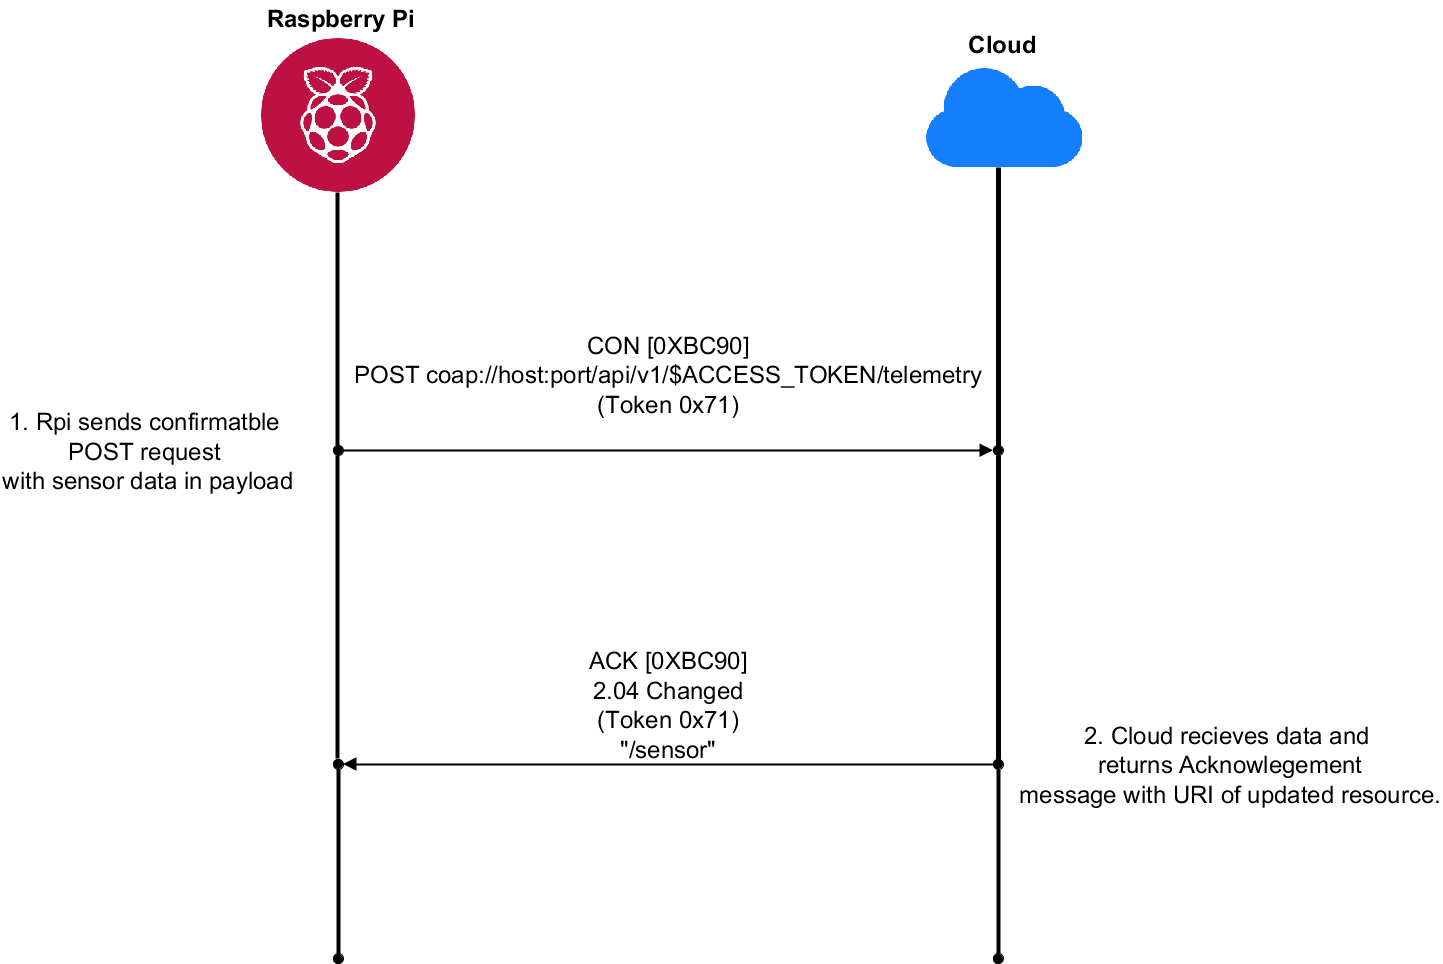
\includegraphics[width=\imageWidth\textwidth]{assets/rpi_cloud_communication.png}
    \caption{\label{fig:rpi_cloud_comms} Diagram showing the communication between \gls{rpi} and the Cloud.}
\end{figure}